\documentclass[light]{lutbeamer}
\usepackage{pgfpages}
\usepackage{ragged2e}
\usepackage{booktabs}
\usepackage{amssymb}
\usepackage{fontawesome5}
\usepackage{tikz}
\usepackage{pgfplots}
\pgfplotsset{compat=1.18}
\addbibresource{references.bib}

% ===================================================================
% METADATA (DERS KIMLIK BILGILERI)
% ===================================================================
\setdepartment{OSTIM Teknik Üniversitesi}
\institute{}
\author[Mühendislik Fakültesi]{\\
Prof.~Dr.~Yalçın ATA \\
Prof.~Dr.~Arif DEMİR \\
Dr.~Öğr.~Üyesi~Emel GÜVEN \\
Dr.~Öğr.~Üyesi~Ufuk ASIL \\
Öğr.~Gör.~Sema ÇİFTÇİ
}
\title{MATH 204 -- Olasılık ve İstatistik}
\subtitle{Hafta 6: Sürekli Olasılık Dağılımları}
\date{2025--2026 Bahar Dönemi}

% ===================================================================
% AUTOMATIC TABLE OF CONTENTS (PRESENTATION FLOW)
% ===================================================================
\setcounter{tocdepth}{2}

\AtBeginSection[]{
  \begin{frame}{Sunum Planı}
    \scriptsize
    \begin{columns}[T]
      \begin{column}{0.48\textwidth}
        \tableofcontents[sections={1-4}, currentsection]
      \end{column}
      \begin{column}{0.48\textwidth}
        \tableofcontents[sections={5-10}, currentsection]
      \end{column}
    \end{columns}
  \end{frame}
}

\begin{document}

\setbeamertemplate{navigation symbols}{}
\setbeamertemplate{footline}{
  \begin{beamercolorbox}[wd=\paperwidth, ht=10pt, dp=1pt]{footline}
    \usebeamerfont{footline}
    \begin{tikzpicture}[remember picture,overlay]
      \node[anchor=south west, xshift=10mm, yshift=.4mm]
      at (current page.south west)
      {\insertshortauthor,~\department};
    \end{tikzpicture}
    \begin{tikzpicture}[remember picture,overlay]
      \node[anchor=south east, xshift=-5mm, yshift=0.5mm]
      at (current page.south east)
      {\insertframenumber \,/\, \inserttotalframenumber};
    \end{tikzpicture}
  \end{beamercolorbox}
}

% ===================================================================
% KAPAK SLAYTLARI
% ===================================================================

% Gorsel Tam Kapak (Logosuz)
\begin{frame}<article:0>[plain,noframenumbering]
  \begin{tikzpicture}[remember picture,overlay]
    \node[anchor=center, at=(current page.center), inner sep=0pt] {
      
\includegraphics[width=\paperwidth, height=\paperheight]{logos/background_figure.jpg}
    };
  \end{tikzpicture}
\end{frame}

% Resmi Baslik Sayfasi (kapak icin ozel alt bilgi)
{
  \setbeamertemplate{footline}{
    \begin{beamercolorbox}[wd=\paperwidth, ht=10pt, dp=1pt]{footline}
      \usebeamerfont{footline}
      \begin{tikzpicture}[remember picture,overlay]
        \node[anchor=south west, xshift=10mm, yshift=.4mm, align=left]
        at (current page.south west)
        {\tiny Bu şablon OTU Yazılım Mühendisliği tarafından hazırlanmış olup \href{https://github.com/ufukasia/Ostim-Teknik--niversitesi-Yaz-l-m-M-hendisli-i---Lutbeamer-egitim-i-eri-i-haz-rlama-}{buradan} güncel haline ulaşabilirsiniz.};
      \end{tikzpicture}
      \begin{tikzpicture}[remember picture,overlay]
        \node[anchor=south east, xshift=-5mm, yshift=0.5mm]
        at (current page.south east)
        {\insertframenumber \,/\, \inserttotalframenumber};
      \end{tikzpicture}
    \end{beamercolorbox}
  }
  \maketitle{}
}

% GENEL ICERIK HARITASI
\begin{frame}{İçindekiler}
  \scriptsize
  \begin{columns}[T]
    \begin{column}{0.48\textwidth}
      \tableofcontents[sections={1-4}]
    \end{column}
    \begin{column}{0.48\textwidth}
      \tableofcontents[sections={5-10}]
    \end{column}
  \end{columns}
\end{frame}

% ===================================================================
% GENEL TEKRAR: MILESTONE TANIMLARI (Hafta 2--5)
% ===================================================================

\section*{Genel Tekrar}

% ------------------------------------------------------------------
% MILESTONE 1: KOŞULLU OLASILIK
% ------------------------------------------------------------------
\begin{frame}{Tekrar 1: Koşullu Olasılık}
    \begin{columns}[T]
        \begin{column}{0.55\textwidth}
            \begin{block}{Tanım}
                $P(B)>0$ olmak koşuluyla, $B$ olayının gerçekleştiği bilindiğinde $A$ olayının olasılığı:
                \[
                P(A|B) = \frac{P(A \cap B)}{P(B)}
                \]
            \end{block}

            \begin{itemize}
                \item \textbf{Pay:} Her iki olayın da birlikte gerçekleşmesi.
                \item \textbf{Payda:} Koşulun olasılığı -- yeni evrenimiz.
                \item Koşullu olasılık da $0 \le P(A|B) \le 1$ aralığındadır.
            \end{itemize}
        \end{column}
        \begin{column}{0.42\textwidth}
            \begin{exampleblock}{Sezgisel Yorum}
                Yeni bilgi geldiğinde örnek uzayımız \textbf{daralır}. Artık $S$ değil, $B$ kümesi yeni evrenimizdir.

                \vspace{0.2cm}
                $A \cap B$ kısımını, $B$'nin içindeki oranına göre normalize ederiz.
            \end{exampleblock}
        \end{column}
    \end{columns}
\end{frame}

\begin{frame}{Özgün Örnek: Koşullu Olasılık}
\small
\begin{columns}[T,onlytextwidth]
    \begin{column}{0.48\textwidth}
        \begin{block}{Soru}
            Bir pil modülü üretim hattında 150 modül termal testi geçmiştir. Bu modüllerin 120 tanesi titreşim testini de geçmiştir.

            \vspace{0.15cm}
            Termal testi geçtiği bilinen bir modülün titreşim testini de geçme olasılığı nedir?
        \end{block}
    \end{column}
    \begin{column}{0.48\textwidth}
        \begin{exampleblock}{Çözüm}
            \[
            P(Ti|Te)=\frac{P(Ti \cap Te)}{P(Te)}
            \]
            Sayım ile:
            \[
            P(Ti|Te)=\frac{120}{150}=0.80
            \]

            Yani termal testi geçen bir modülün titreşim testini de geçme olasılığı \%80'dir.
        \end{exampleblock}
    \end{column}
\end{columns}
\end{frame}

% ------------------------------------------------------------------
% MILESTONE 2: ÇARPIM KURALI
% ------------------------------------------------------------------
\begin{frame}[fragile]
    \frametitle{Tekrar 2: Çarpım Kuralı}
    \begin{block}{İki Olay İçin}
        Koşullu olasılık tanımından:
        \[
        P(A \cap B) = P(B) \cdot P(A|B) = P(A) \cdot P(B|A)
        \]
    \end{block}

    \begin{block}{Zincir Kuralı ($k$ Olay)}
        \[
        P(A_1 \cap A_2 \cap \cdots \cap A_k)
        = P(A_1)\, P(A_2|A_1)\, P(A_3|A_1 \cap A_2) \cdots
        \]
    \end{block}

    \begin{exampleblock}{Uygulama Alanı}
        Yerine koymadan çekim problemlerinde (kart, sigorta, top çekme) her adımda havuz küçülür; koşullu olasılıklar buna göre güncellenir.
    \end{exampleblock}
\end{frame}

\begin{frame}{Özgün Örnek: Çarpım Kuralı}
\small
\begin{columns}[T,onlytextwidth]
    \begin{column}{0.48\textwidth}
        \begin{block}{Soru}
            Bir kontrol kartının optik incelemeyi geçme olasılığı 0.93'tür. Optik incelemeyi geçen kartların fonksiyonel testi geçme olasılığı 0.96'dır.

            \vspace{0.15cm}
            Kartın iki testi de geçme olasılığı nedir?
        \end{block}
    \end{column}
    \begin{column}{0.48\textwidth}
        \begin{exampleblock}{Çözüm}
            \[
            P(O \cap F)=P(O)\,P(F|O)
            \]
            \[
            =0.93 \times 0.96 = 0.8928
            \]

            Sonuç olarak kartın iki testi de geçme olasılığı yaklaşık \%89.28'dir.
        \end{exampleblock}
    \end{column}
\end{columns}
\end{frame}

% ------------------------------------------------------------------
% MILESTONE 3: BAĞIMSIZLIK
% ------------------------------------------------------------------
\begin{frame}{Tekrar 3: Bağımsızlık}
    \begin{columns}[T]
        \begin{column}{0.48\textwidth}
            \begin{block}{Tanım}
                İki olay $A$ ve $B$ \textbf{bağımsızdır} $\iff$
                \[
                P(A \cap B) = P(A)\, P(B)
                \]
                Eşdeğer ifade: $P(A|B) = P(A)$.
            \end{block}

            \begin{itemize}
                \item $B$'yi bilmek, $A$'nın olasılığını \textbf{değiştirmez}.
                \item $A$ ve $B$ bağımsızsa $\Rightarrow$ $A'$ ve $B$ de bağımsızdır.
            \end{itemize}
        \end{column}
        \begin{column}{0.48\textwidth}
            \begin{alertblock}{Dikkat: Ayrıklık $\neq$ Bağımsızlık}
                \textbf{Ayrık:} $A \cap B = \emptyset$ $\Rightarrow$ $P(A \cap B)=0$.

                \vspace{0.15cm}
                İki pozitif olasılıklı olay hem ayrık hem bağımsız \textbf{olamaz}; çünkü $P(A)P(B) > 0 \neq 0$.
            \end{alertblock}
        \end{column}
    \end{columns}
\end{frame}

\begin{frame}{Özgün Örnek: Bağımsızlık}
\small
\begin{columns}[T,onlytextwidth]
    \begin{column}{0.48\textwidth}
        \begin{block}{Soru}
            Bir veri merkezinde iki bağımsız yedek güç ünitesi vardır.

            \[
            P(A)=0.98, \qquad P(B)=0.95
            \]

            İki ünitenin aynı anda çalışır durumda olma olasılığı nedir?
        \end{block}
    \end{column}
    \begin{column}{0.48\textwidth}
        \begin{exampleblock}{Çözüm}
            Olaylar bağımsız olduğu için:
            \[
            P(A \cap B)=P(A)P(B)
            \]
            \[
            =0.98 \times 0.95 = 0.931
            \]

            Yani iki yedek ünitenin birlikte hazır olma olasılığı \%93.1'dir.
        \end{exampleblock}
    \end{column}
\end{columns}
\end{frame}

\begin{frame}{Soru 15: Sistem Güvenilirliği}
\scriptsize
\begin{columns}[T,onlytextwidth]
    \begin{column}{0.48\textwidth}
        \begin{block}{Soru}
            Paralel bağlı 3 bileşenli bir elektrik sisteminde, sistem en az bir bileşen çalıştığı sürece çalışmaktadır.

            \vspace{0.15cm}
            $t$ zamanından önce arızalanma olasılıkları:
            \[
            P(F_1)=0.1,\quad P(F_2)=0.2,\quad P(F_3)=0.3
            \]
            ve ömürler bağımsızdır.

            \vspace{0.15cm}
            Sistemin $t$ zamanından önce arızalanma olasılığı nedir?
        \end{block}
    \end{column}
    \begin{column}{0.48\textwidth}
        \begin{exampleblock}{Çözüm}
            Paralel sistem ancak \textbf{tüm} bileşenler arızalanırsa durur:
            \[
            P(F_{\text{sistem}})=P(F_1 \cap F_2 \cap F_3)
            \]

            Bağımsızlıktan:
            \[
            =0.1 \times 0.2 \times 0.3 = 0.006
            \]

            Yani sistemin $t$ zamanından önce arızalanma olasılığı
            \[
            0.006 = \%0.6
            \]
            olur.
        \end{exampleblock}
    \end{column}
\end{columns}
\end{frame}

% ------------------------------------------------------------------
% MILESTONE 4: TOPLAM OLASILIK TEOREMİ
% ------------------------------------------------------------------
\begin{frame}[fragile]
    \frametitle{Tekrar 4: Toplam Olasılık Teoremi}
    \begin{columns}[T]
        \begin{column}{0.55\textwidth}
            \begin{block}{Teorem}
                $B_1, B_2, \dots, B_k$ örneklem uzayının bir bölüntüsü ise:
                \[
                P(A) = \sum_{i=1}^{k} P(B_i)\, P(A|B_i)
                \]
            \end{block}

            \begin{itemize}
                \item Her terim bir ``dal olasılığı'': Kaynağın ağırlığı $\times$ o kaynaktan $A$ çıkma oranı.
                \item Tüm dalların toplamı $A$'nın genel olasılığını verir.
            \end{itemize}
        \end{column}
        \begin{column}{0.42\textwidth}
            \centering
            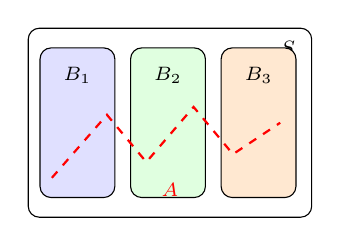
\begin{tikzpicture}[x=1cm,y=1cm,every node/.style={font=\scriptsize}]
                \draw[rounded corners] (0,0) rectangle (3.6,2.4);
                \node at (3.3,2.15) {$S$};
                \draw[fill=blue!12,rounded corners] (0.15,0.25) rectangle (1.1,2.15);
                \draw[fill=green!12,rounded corners] (1.3,0.25) rectangle (2.25,2.15);
                \draw[fill=orange!18,rounded corners] (2.45,0.25) rectangle (3.4,2.15);
                \node at (0.625,1.8) {$B_1$};
                \node at (1.775,1.8) {$B_2$};
                \node at (2.925,1.8) {$B_3$};
                \draw[thick, red, dashed] (0.3,0.5) -- (1.0,1.3) -- (1.5,0.7) -- (2.1,1.4) -- (2.6,0.8) -- (3.2,1.2);
                \node[red] at (1.8,0.35) {$A$};
            \end{tikzpicture}

            \vspace{0.2cm}
            \scriptsize $A$, farklı kaynaklardan ($B_i$) gelen parçaların birleşimidir.
        \end{column}
    \end{columns}
\end{frame}

\begin{frame}{Özgün Örnek: Toplam Olasılık}
\small
\begin{columns}[T,onlytextwidth]
    \begin{column}{0.48\textwidth}
        \begin{block}{Soru}
            Üç üretim hattı günlük üretimin sırasıyla \%50, \%30 ve \%20'sini yapıyor.

            Hurda oranları:
            \[
            P(H|A)=0.02,\; P(H|B)=0.03,\; P(H|C)=0.05
            \]

            Rastgele seçilen bir parçanın hurdalı olma olasılığı nedir?
        \end{block}
    \end{column}
    \begin{column}{0.48\textwidth}
        \begin{exampleblock}{Çözüm}
            \[
            P(H)=\sum_i P(B_i)P(H|B_i)
            \]
            \[
            =0.50(0.02)+0.30(0.03)+0.20(0.05)
            \]
            \[
            =0.010+0.009+0.010=0.029
            \]

            Genel hurda olasılığı \%2.9'dur.
        \end{exampleblock}
    \end{column}
\end{columns}
\end{frame}

% ------------------------------------------------------------------
% MILESTONE 5: BAYES TEOREMİ
% ------------------------------------------------------------------
\begin{frame}[fragile]
    \frametitle{Tekrar 5: Bayes Teoremi}
    \begin{block}{Teorem}
        $B_1, \dots, B_k$ bir bölüntü ve $P(A) > 0$ olsun. Gözlem $A$ yapıldığında, bunun $r$'inci kaynaktan gelme olasılığı:
        \[
        P(B_r | A) = \frac{P(B_r)\, P(A|B_r)}{\displaystyle\sum_{i=1}^{k} P(B_i)\, P(A|B_i)}
        \]
    \end{block}

    \begin{columns}[T]
        \begin{column}{0.48\textwidth}
            \begin{exampleblock}{Okuma Yöntemi}
                \begin{itemize}
                    \item \textbf{Pay:} $r$'inci dalın katkısı.
                    \item \textbf{Payda:} Toplam Olasılık ($P(A)$).
                    \item Sonuçtan sebebe giden yol.
                \end{itemize}
            \end{exampleblock}
        \end{column}
        \begin{column}{0.48\textwidth}
            \begin{alertblock}{En Sık Yapılan Hata}
                \[
                P(A|B) \neq P(B|A)
                \]
                Bayes teoremi bu iki yönü birbirine dönüştürme aracıdır.
            \end{alertblock}
        \end{column}
    \end{columns}
\end{frame}

\begin{frame}{Özgün Örnek: Bayes Teoremi}
\small
\begin{columns}[T,onlytextwidth]
    \begin{column}{0.48\textwidth}
        \begin{block}{Soru}
            Az önceki üç üretim hattında hurdalı bir parça bulunduğunda, bu parçanın C hattından gelmiş olma olasılığı nedir?

            \vspace{0.15cm}
            \[
            P(C)=0.20,\quad P(H|C)=0.05,\quad P(H)=0.029
            \]
        \end{block}
    \end{column}
    \begin{column}{0.48\textwidth}
        \begin{exampleblock}{Çözüm}
            \[
            P(C|H)=\frac{P(C)P(H|C)}{P(H)}
            \]
            \[
            =\frac{0.20 \times 0.05}{0.029}
            =\frac{0.010}{0.029}\approx 0.345
            \]

            Hurdalı parçanın C hattından gelmiş olma olasılığı yaklaşık \%34.5'tir.
        \end{exampleblock}
    \end{column}
\end{columns}
\end{frame}

% ------------------------------------------------------------------
% MILESTONE 6: RASTGELE DEĞİŞKEN
% ------------------------------------------------------------------
\begin{frame}{Tekrar 6: Rastgele Değişken Kavramı}
    \begin{columns}[T]
        \begin{column}{0.55\textwidth}
            \begin{block}{Tanım}
                Rastgele değişken, örnek uzaydaki \textbf{her elemana bir reel sayı atayan} fonksiyondur:
                \[
                X : S \to \mathbb{R}, \qquad \omega \mapsto X(\omega).
                \]
            \end{block}

            \begin{itemize}
                \item $X$: Değişkenin adı (büyük harf).
                \item $x$: Aldığı belirli bir değer (küçük harf).
                \item Olayları sayılara çevirerek \textbf{istatistiğe köprü} kurar.
            \end{itemize}
        \end{column}
        \begin{column}{0.42\textwidth}
            \begin{exampleblock}{İki Temel Tür}
                \begin{itemize}
                    \item \textbf{Ayrık:} Değer kümesi sayılabilir.

                    $X \in \{0,1,2,\dots\}$ (adet, sayım).
                    \item \textbf{Sürekli:} Değer kümesi bir aralık.

                    $X \in [a,b]$ (ölçüm, süre).
                \end{itemize}
            \end{exampleblock}
        \end{column}
    \end{columns}
\end{frame}

\begin{frame}{Özgün Örnek: Rastgele Değişken Tanımlama}
\small
\begin{columns}[T,onlytextwidth]
    \begin{column}{0.48\textwidth}
        \begin{block}{Soru}
            Bir baskı devre kartında 4 kritik lehim noktası kontrol ediliyor.

            \vspace{0.15cm}
            $X=$ ``hatalı lehim noktası sayısı'' olarak tanımlansın.

            \vspace{0.15cm}
            $X$ hangi değerleri alabilir ve türü nedir?
        \end{block}
    \end{column}
    \begin{column}{0.48\textwidth}
        \begin{exampleblock}{Çözüm}
            Hatalı lehim sayısı:
            \[
            X \in \{0,1,2,3,4\}
            \]

            Bu değer kümesi sayılabilir olduğu için $X$ bir \textbf{ayrık rastgele değişken}dir.

            \vspace{0.15cm}
            Burada olayları sayıya çevirmiş olduk.
        \end{exampleblock}
    \end{column}
\end{columns}
\end{frame}

\begin{frame}{Soru 6: Paradan Türetilen Rastgele Değişken}
\scriptsize
\begin{columns}[T,onlytextwidth]
    \begin{column}{0.48\textwidth}
        \begin{block}{Soru}
            Bir madeni para 4 kez atılıyor.

            \vspace{0.15cm}
            $W$, yazı sayısından tura sayısının çıkarılmasıyla tanımlanıyor:
            \[
            W = H - T
            \]

            $W$'nin alabileceği olası değerleri listeleyiniz.
        \end{block}
    \end{column}
    \begin{column}{0.48\textwidth}
        \begin{exampleblock}{Çözüm}
            Yazı sayısı $H$ olsun. O zaman $H \in \{0,1,2,3,4\}$ ve tura sayısı $4-H$ olur.

            \[
            W = H-(4-H)=2H-4
            \]

            Buna göre:
            \[
            W \in \{-4,-2,0,2,4\}
            \]
        \end{exampleblock}
    \end{column}
\end{columns}
\end{frame}

\begin{frame}{Soru 10: Vale Problemi ve Olası Değerler}
\scriptsize
\begin{columns}[T,onlytextwidth]
    \begin{column}{0.48\textwidth}
        \begin{block}{Soru}
            Bir vale, Alice, Bob ve Charlie'ye ait 3 anahtarı karıştırıyor ve anahtarları rastgele geri veriyor.

            \vspace{0.15cm}
            Doğru anahtarı alan müşteri sayısını gösteren rastgele değişken $M$ olsun.

            \vspace{0.15cm}
            $M$'nin alabileceği olası değerler nelerdir?
        \end{block}
    \end{column}
    \begin{column}{0.48\textwidth}
        \begin{exampleblock}{Çözüm}
            Olası doğru eşleşme sayıları:
            \[
            M=0,\;1,\;3
            \]

            \vspace{0.15cm}
            \textbf{$M=2$ mümkün değildir}; çünkü iki kişi doğru anahtarı alırsa üçüncü kişi de otomatik olarak doğru anahtarı almış olur.

            \vspace{0.15cm}
            Dolayısıyla:
            \[
            M \in \{0,1,3\}
            \]
        \end{exampleblock}
    \end{column}
\end{columns}
\end{frame}

% ------------------------------------------------------------------
% MILESTONE 7: OLASILIK KÜTLE FONKSİYONU (PMF)
% ------------------------------------------------------------------
\begin{frame}[fragile]
    \frametitle[PMF]{Tekrar 7: Olasılık Kütle Fonksiyonu (PMF)}
    \begin{block}{Tanım}
        Ayrık rastgele değişken $X$'in olasılık fonksiyonu $f(x)=P(X=x)$ şu koşulları sağlar:
        \begin{enumerate}
            \item $f(x) \ge 0$ \quad (negatif olasılık yoktur).
            \item $\displaystyle\sum_x f(x) = 1$ \quad (tüm olasılıklar toplamı 1'dir).
        \end{enumerate}
    \end{block}

    \begin{columns}[T]
        \begin{column}{0.48\textwidth}
            \begin{exampleblock}{Tablo Örneği}
                \centering
                \begin{tabular}{cccc}
                    \toprule
                    $x$ & 0 & 1 & 2 \\
                    \midrule
                    $f(x)$ & $1/4$ & $1/2$ & $1/4$ \\
                    \bottomrule
                \end{tabular}

                \vspace{0.1cm}
                \scriptsize Kontrol: $1/4 + 1/2 + 1/4 = 1$ \;\checkmark
            \end{exampleblock}
        \end{column}
        \begin{column}{0.48\textwidth}
            \begin{alertblock}{Dikkat}
                PMF yalnızca \textbf{ayrık} değişkenlerde tanımlıdır. Sürekli değişkenlerde $P(X=x) = 0$ olduğundan bunun yerine \textbf{yoğunluk fonksiyonu (PDF)} kullanılır.
            \end{alertblock}
        \end{column}
    \end{columns}
\end{frame}

\begin{frame}{Özgün Örnek: PMF ile Olasılık}
\small
\begin{columns}[T,onlytextwidth]
    \begin{column}{0.48\textwidth}
        \begin{block}{Soru}
            Bir mobil robotun vardiya başına arıza sayısı için
            \[
            \begin{aligned}
            P(X=0)&=0.50 \\
            P(X=1)&=0.30 \\
            P(X=2)&=0.20
            \end{aligned}
            \]
            veriliyor.

            \vspace{0.15cm}
            En az bir arıza görülme olasılığı nedir?
        \end{block}
    \end{column}
    \begin{column}{0.48\textwidth}
        \begin{exampleblock}{Çözüm}
            \[
            P(X \ge 1)=P(X=1)+P(X=2)
            \]
            \[
            =0.30+0.20=0.50
            \]

            Alternatif olarak:
            \[
            P(X \ge 1)=1-P(X=0)=1-0.50=0.50
            \]
        \end{exampleblock}
    \end{column}
\end{columns}
\end{frame}

\begin{frame}{Soru 7: Sabit $c$ ile PMF Kurma}
\scriptsize
\begin{columns}[T,onlytextwidth]
    \begin{column}{0.48\textwidth}
        \begin{block}{Soru}
            Aşağıdaki fonksiyonun bir olasılık dağılımı olabilmesi için $c$ değerini bulunuz:
            \[
            f(x)=c(x^2+4), \qquad x=0,1,2,3
            \]
        \end{block}
    \end{column}
    \begin{column}{0.48\textwidth}
        \begin{exampleblock}{Çözüm}
            PMF için toplam 1 olmalıdır:
            \[
            \sum_{x=0}^{3} c(x^2+4)=1
            \]
            \[
            c[(0+1+4+9)+4+4+4+4]=1
            \]
            \[
            30c=1 \quad \Rightarrow \quad c=\frac{1}{30}
            \]
        \end{exampleblock}
    \end{column}
\end{columns}
\end{frame}

\begin{frame}{Soru 11: Rekürsif PMF'den Kapalı Form}
\scriptsize
\begin{columns}[T,onlytextwidth]
    \begin{column}{0.48\textwidth}
        \begin{block}{Soru}
            Ayrık rastgele değişken $X$, $x=1,2,3,\ldots$ değerlerini almakta ve
            \[
            P(X=x+1)=\frac{1}{3}P(X=x), \qquad x \ge 1
            \]
            bağıntısını sağlamaktadır.

            \vspace{0.15cm}
            $P(X=x)$ için kapalı form ifadeyi bulunuz.
        \end{block}
    \end{column}
    \begin{column}{0.48\textwidth}
        \begin{exampleblock}{Çözüm}
            $P(X=1)=a$ olsun. O zaman
            \[
            P(X=x)=a\left(\frac{1}{3}\right)^{x-1}, \qquad x \ge 1
            \]

            Normalize edersek:
            \[
            1=\sum_{x=1}^{\infty} a\left(\frac{1}{3}\right)^{x-1}
            =a\frac{1}{1-\frac{1}{3}}=\frac{3a}{2}
            \]
            \[
            a=\frac{2}{3}
            \]

            Sonuç:
            \[
            P(X=x)=\frac{2}{3^x}, \qquad x=1,2,3,\ldots
            \]
        \end{exampleblock}
    \end{column}
\end{columns}
\end{frame}

\begin{frame}{Soru 12: Logaritmik PMF Özelliği}
\scriptsize
\begin{columns}[T,onlytextwidth]
    \begin{column}{0.48\textwidth}
        \begin{block}{Soru}
            $p\in(-1,0)$ için
            \[
            p(x)=c\frac{(-1)^{x-1}}{x}p^x, \qquad x \ge 1
            \]
            şeklinde verilen PMF'de $c$ sabitini bulunuz.
        \end{block}
    \end{column}
    \begin{column}{0.48\textwidth}
        \begin{exampleblock}{Çözüm}
            Toplam 1 olmalıdır:
            \[
            1=c\sum_{x=1}^{\infty}\frac{(-1)^{x-1}p^x}{x}
            \]

            Bilinen seri:
            \[
            \sum_{x=1}^{\infty}\frac{(-1)^{x-1}p^x}{x}=\ln(1+p)
            \]

            Dolayısıyla:
            \[
            c\,\ln(1+p)=1
            \]
            \[
            c=\frac{1}{\ln(1+p)}
            \]
        \end{exampleblock}
    \end{column}
\end{columns}
\end{frame}

\begin{frame}{Soru 2: Sonsuz Serili PMF}
\scriptsize
\begin{columns}[T,onlytextwidth]
    \begin{column}{0.48\textwidth}
        \begin{block}{Soru}
            Ayrık bir rastgele değişken için
            \[
            p(x)=c\frac{2^x}{x!}, \qquad x=0,1,2,\ldots
            \]
            veriliyor.

            \vspace{0.15cm}
            \begin{enumerate}
                \item $c$ sabitini bulunuz.
                \item $P(X \ge 2)$ olasılığını hesaplayınız.
            \end{enumerate}
        \end{block}
    \end{column}
    \begin{column}{0.48\textwidth}
        \begin{exampleblock}{Çözüm}
            \[
            1=c\sum_{x=0}^{\infty}\frac{2^x}{x!}=c\,e^2
            \quad \Rightarrow \quad
            c=e^{-2}
            \]

            Sonra:
            \[
            P(X \ge 2)=1-P(X=0)-P(X=1)
            \]
            \[
            =1-c(1)-c(2)=1-3e^{-2}
            \]

            Yani:
            \[
            P(X \ge 2)=1-3e^{-2}\approx 0.594
            \]
        \end{exampleblock}
    \end{column}
\end{columns}
\end{frame}

\begin{frame}{Soru 1: Torbadan 4 Pul Çekimi}
\scriptsize
\begin{block}{Soru}
    Bir torbada 6 kırmızı, 5 beyaz ve 8 mavi pul vardır. Geri koymadan rastgele 4 pul seçiliyor.

    \vspace{0.15cm}
    Seçilen kırmızı pul sayısını gösteren rastgele değişken $X$ olsun.

    \vspace{0.15cm}
    \begin{enumerate}
        \item $X$'in olasılık kütle fonksiyonunu bulunuz.
        \item En az bir kırmızı pul çekilmesi olasılığını hesaplayınız.
    \end{enumerate}
\end{block}
\end{frame}

\begin{frame}{Soru 1: Çözüm}
\scriptsize
\begin{block}{PMF}
    Toplam pul sayısı $19$, kırmızı dışı pul sayısı $13$ olduğundan:
    \[
    f(x)=P(X=x)=\frac{\binom{6}{x}\binom{13}{4-x}}{\binom{19}{4}},
    \qquad x=0,1,2,3,4
    \]
\end{block}

\begin{block}{En Az Bir Kırmızı}
    \[
    P(X \ge 1)=1-P(X=0)
    \]
    \[
    =1-\frac{\binom{6}{0}\binom{13}{4}}{\binom{19}{4}}
    =1-\frac{\binom{13}{4}}{\binom{19}{4}}
    \]
    \[
    =1-\frac{715}{3876}
    =\frac{3161}{3876}\approx 0.8155
    \]
\end{block}
\end{frame}

\begin{frame}{Soru 3: Arızalı Dizüstü Bilgisayarlar}
\scriptsize
\begin{columns}[T,onlytextwidth]
    \begin{column}{0.48\textwidth}
        \begin{block}{Soru}
            20 dizüstü bilgisayardan oluşan bir sevkiyatta 3 bilgisayar arızalıdır. Bir okul rastgele 2 tane satın alıyor.

            \vspace{0.15cm}
            Satın alınan arızalı bilgisayar sayısını gösteren rastgele değişken $X$ için PMF'yi bulunuz.
        \end{block}
    \end{column}
    \begin{column}{0.48\textwidth}
        \begin{exampleblock}{Çözüm}
            Bu bir hipergeometrik dağılımdır:
            \[
            f(x)=\frac{\binom{3}{x}\binom{17}{2-x}}{\binom{20}{2}},
            \qquad x=0,1,2
            \]

            \[
            f(0)=\frac{136}{190},\quad
            f(1)=\frac{51}{190},\quad
            f(2)=\frac{3}{190}
            \]
        \end{exampleblock}
    \end{column}
\end{columns}
\end{frame}

\begin{frame}{Soru 4: Yan Hava Yastıklı Araç Sayısı}
\scriptsize
\begin{columns}[T,onlytextwidth]
    \begin{column}{0.48\textwidth}
        \begin{block}{Soru}
            Bir otomobil galerisi sattığı araçların \%50'sini yan hava yastıklı satmaktadır.

            \vspace{0.15cm}
            $X$, satılan sonraki 4 araç arasında yan hava yastığı bulunan araç sayısı olsun.

            \vspace{0.15cm}
            $f(x)$ dağılım fonksiyonunu yazınız.
        \end{block}
    \end{column}
    \begin{column}{0.48\textwidth}
        \begin{exampleblock}{Çözüm}
            \[
            X \sim Bin(4,0.5)
            \]
            Bu yüzden:
            \[
            f(x)=P(X=x)=\binom{4}{x}(0.5)^x(0.5)^{4-x}
            \]
            \[
            =\frac{\binom{4}{x}}{16},
            \qquad x=0,1,2,3,4
            \]
        \end{exampleblock}
    \end{column}
\end{columns}
\end{frame}

\begin{frame}{Soru 8: PMF'den Koşullu Olasılık}
\scriptsize
\begin{columns}[T,onlytextwidth]
    \begin{column}{0.48\textwidth}
        \begin{block}{Soru}
            $X$, bir işlemcideki hata sayısını göstersin:
            \[
            P(X=x)=k(4-x), \qquad x\in\{0,1,2,3\}
            \]

            \vspace{0.15cm}
            En az bir hata olduğu biliniyorsa, tam olarak 2 hata bulunması olasılığı nedir?
        \end{block}
    \end{column}
    \begin{column}{0.48\textwidth}
        \begin{exampleblock}{Çözüm}
            Önce $k$ bulunur:
            \[
            k(4+3+2+1)=1 \Rightarrow 10k=1 \Rightarrow k=\frac{1}{10}
            \]

            \[
            P(X=2)=\frac{2}{10}, \qquad P(X \ge 1)=1-\frac{4}{10}=\frac{6}{10}
            \]

            \[
            P(X=2|X \ge 1)=\frac{2/10}{6/10}=\frac{1}{3}
            \]
        \end{exampleblock}
    \end{column}
\end{columns}
\end{frame}

\begin{frame}{Soru 13: $Z=\max(X,Y)$ için PMF}
\scriptsize
\begin{columns}[T,onlytextwidth]
    \begin{column}{0.48\textwidth}
        \begin{block}{Soru}
            $X$ ve $Y$, $\{1,2,3,4,5,6\}$ üzerinde düzgün dağılan bağımsız ayrık rastgele değişkenler olsun.

            \vspace{0.15cm}
            \[
            Z=\max(X,Y)
            \]
            için PMF'yi bulunuz.
        \end{block}
    \end{column}
    \begin{column}{0.48\textwidth}
        \begin{exampleblock}{Çözüm}
            Önce:
            \[
            P(Z \le z)=P(X \le z,\;Y \le z)=\left(\frac{z}{6}\right)^2
            \]
            \[
            z=1,2,\ldots,6
            \]

            Bu yüzden:
            \[
            P(Z=z)=P(Z \le z)-P(Z \le z-1)
            \]
            \[
            =\frac{z^2-(z-1)^2}{36}
            =\frac{2z-1}{36}, \qquad z=1,\ldots,6
            \]
        \end{exampleblock}
    \end{column}
\end{columns}
\end{frame}

\begin{frame}{Soru 14: Negatif Binom Kavram Kontrolü}
\scriptsize
\begin{block}{Soru}
    Bir kalite kontrol sürecinde bileşenler bağımsız olarak test ediliyor.

    \vspace{0.15cm}
    Testi geçme olasılığı $0.8$, başarısız olma olasılığı $0.2$'dir. Tam olarak 3 başarısızlık kaydedilene kadar teste devam ediliyor.

    \vspace{0.15cm}
    Toplam test edilen bileşen sayısını gösteren rastgele değişken $N$ için
    \begin{enumerate}
        \item genel PMF ifadesini,
        \item $P(N=5)$ olasılığını
    \end{enumerate}
    bulunuz.
\end{block}
\end{frame}

\begin{frame}{Soru 14: Çözüm}
\scriptsize
\begin{block}{Genel PMF}
    Üçüncü başarısızlığın $n$'inci denemede gelmesi için, ilk $n-1$ denemede tam 2 başarısızlık olmalıdır:
    \[
    P(N=n)=\binom{n-1}{2}(0.2)^3(0.8)^{n-3},
    \qquad n=3,4,5,\ldots
    \]
\end{block}

\begin{block}{$P(N=5)$}
    \[
    P(N=5)=\binom{4}{2}(0.2)^3(0.8)^2
    \]
    \[
    =6 \times 0.008 \times 0.64 = 0.03072
    \]
\end{block}
\end{frame}

% ------------------------------------------------------------------
% MILESTONE 8: BİRİKİMLİ DAĞILIM FONKSİYONU (CDF)
% ------------------------------------------------------------------
\begin{frame}[fragile]
    \frametitle[CDF]{Tekrar 8: Birikimli Dağılım Fonksiyonu (CDF)}
    \small
    \begin{block}{Tanım}
        Rastgele değişken $X$'in belirli bir $x$ değerine eşit veya daha küçük olma olasılıklarının toplamıdır:
        \[
        F(x) = P(X \le x) = \sum_{t \le x} f(t), \qquad -\infty < x < \infty
        \]
    \end{block}

    \begin{columns}[T]
        \begin{column}{0.48\textwidth}
            \begin{exampleblock}{Kumbara Mantığı}
                \begin{itemize}
                    \item CDF, soldan sağa doğru olasılıkları \textbf{üst üste ekler}.
                    \item Hiçbir zaman azalmaz (basamak fonksiyonu).
                    \item $F(-\infty) = 0$, \; $F(\infty) = 1$.
                \end{itemize}
            \end{exampleblock}
        \end{column}
        \begin{column}{0.48\textwidth}
            \begin{block}{Aralık Olasılığı}
                CDF biliniyorsa:
                \[
                P(a < X \le b) = F(b) - F(a)
                \]
                Geriye dönüş:
                \[
                f(x) = F(x) - F(x^{-})
                \]
            \end{block}
        \end{column}
    \end{columns}
\end{frame}

\begin{frame}{Özgün Örnek: CDF ile Hızlı Hesap}
\small
\begin{columns}[T,onlytextwidth]
    \begin{column}{0.48\textwidth}
        \begin{block}{Soru}
            Bir ağ cihazında günlük paket kaybı sayısı için
            \[
            \begin{aligned}
            P(X=0)&=0.20 \\
            P(X=1)&=0.50 \\
            P(X=2)&=0.30
            \end{aligned}
            \]
            veriliyor.
            \[
            F(1)=P(X \le 1)
            \]
            ve
            \[
            P(1 < X \le 2)
            \]
            nedir?
        \end{block}
    \end{column}
    \begin{column}{0.48\textwidth}
        \begin{exampleblock}{Çözüm}
            \[
            F(1)=P(X=0)+P(X=1)=0.20+0.50=0.70
            \]
            \[
            P(1 < X \le 2)=F(2)-F(1)=1-0.70=0.30
            \]

            CDF birikimli hesap yapmayı hızlandırır.
        \end{exampleblock}
    \end{column}
\end{columns}
\end{frame}

\begin{frame}{Soru 5: Birikimli Dağılım Fonksiyonu}
\scriptsize
\begin{columns}[T,onlytextwidth]
    \begin{column}{0.48\textwidth}
        \begin{block}{Soru}
            4. sorudaki dağılıma göre, satılan sonraki 4 aracın en fazla 2 tanesinde yan hava yastığı bulunması olasılığı nedir?

            \vspace{0.15cm}
            Yani:
            \[
            F(2)=P(X \le 2)
            \]
            değerini bulunuz.
        \end{block}
    \end{column}
    \begin{column}{0.48\textwidth}
        \begin{exampleblock}{Çözüm}
            $X \sim Bin(4,0.5)$ olduğundan:
            \[
            F(2)=\sum_{x=0}^{2}\binom{4}{x}(0.5)^4
            \]
            \[
            =\frac{\binom{4}{0}+\binom{4}{1}+\binom{4}{2}}{16}
            \]
            \[
            =\frac{1+4+6}{16}=\frac{11}{16}=0.6875
            \]
        \end{exampleblock}
    \end{column}
\end{columns}
\end{frame}

\begin{frame}{Soru 9: CDF'den Yeni Bir Değişken Türetme}
\scriptsize
\begin{block}{Soru}
    Ayrık rastgele değişken $X$'in CDF'si
    \[
    F(x)=
    \begin{cases}
    0, & x<1,\\
    0.1, & 1\le x<3,\\
    0.4, & 3\le x<5,\\
    0.8, & 5\le x<7,\\
    1.0, & x\ge 7
    \end{cases}
    \]
    olarak veriliyor. $Y=X^2-10$ olsun. $Y$'nin PMF'sini bulunuz.
\end{block}
\end{frame}

\begin{frame}{Soru 9: Çözüm}
\scriptsize
\begin{block}{Önce $X$'in PMF'si}
    CDF'deki sıçramalardan:
    \[
    P(X=1)=0.1,\quad P(X=3)=0.3,\quad P(X=5)=0.4,\quad P(X=7)=0.2
    \]
\end{block}

\begin{block}{Sonra $Y=X^2-10$}
    \[
    \begin{array}{c|cccc}
    X & 1 & 3 & 5 & 7 \\ \hline
    Y=X^2-10 & -9 & -1 & 15 & 39
    \end{array}
    \]

    Dolayısıyla:
    \[
    P(Y=-9)=0.1,\;
    P(Y=-1)=0.3,\;
    P(Y=15)=0.4,\;
    P(Y=39)=0.2
    \]
\end{block}
\end{frame}

% ------------------------------------------------------------------
% MILESTONE 9: BEKLENEN DEĞER
% ------------------------------------------------------------------
\begin{frame}[fragile]
    \frametitle{Tekrar 9: Beklenen Değer (Matematiksel Beklenti)}
    \begin{columns}[T]
        \begin{column}{0.48\textwidth}
            \begin{block}{Kesikli}
                \[
                \mu = E(X) = \sum_x x\, f(x)
                \]
            \end{block}

            \begin{block}{Sürekli}
                \[
                \mu = E(X) = \int_{-\infty}^{\infty} x\, f(x)\, dx
                \]
            \end{block}
        \end{column}
        \begin{column}{0.48\textwidth}
            \begin{exampleblock}{Ne İfade Eder?}
                Dağılımın \textbf{ağırlık merkezi}dir. Deney sonsuz kez tekrarlanırsa, gözlemlerin aritmetik ortalaması bu değere yakınsar.
            \end{exampleblock}

            \begin{block}{$g(X)$'in Beklenen Değeri}
                \[
                E[g(X)] = \sum_x g(x)\, f(x)
                \]
                Yeni bir dağılım türetmeye \textbf{gerek yoktur}.
            \end{block}
        \end{column}
    \end{columns}
\end{frame}

\begin{frame}{Özgün Örnek: Beklenen Değer}
\small
\begin{columns}[T,onlytextwidth]
    \begin{column}{0.48\textwidth}
        \begin{block}{Soru}
            Bir sensör kartı için yeniden işleme sayısı $X$ şu dağılıma sahip olsun:
            \[
            \begin{aligned}
            P(X=0)&=0.60 \\
            P(X=1)&=0.30 \\
            P(X=2)&=0.10
            \end{aligned}
            \]

            \vspace{0.15cm}
            Beklenen yeniden işleme sayısı nedir?
        \end{block}
    \end{column}
    \begin{column}{0.48\textwidth}
        \begin{exampleblock}{Çözüm}
            \[
            E(X)=\sum x f(x)
            \]
            \[
            =0(0.60)+1(0.30)+2(0.10)
            \]
            \[
            =0+0.30+0.20=0.50
            \]

            Uzun vadede kart başına ortalama yeniden işleme sayısı 0.50'dir.
        \end{exampleblock}
    \end{column}
\end{columns}
\end{frame}

% ------------------------------------------------------------------
% MILESTONE 10: VARYANS VE STANDART SAPMA
% ------------------------------------------------------------------
\begin{frame}[fragile]
    \frametitle{Tekrar 10: Varyans ve Standart Sapma}
    \scriptsize
    \begin{block}{Tanım}
        Değerlerin ortalamadan sapmalarının karesinin beklenen değeridir:
        \[
        \sigma^2 = Var(X) = E\bigl[(X - \mu)^2\bigr]
        \]
    \end{block}

    \begin{columns}[T]
        \begin{column}{0.48\textwidth}
            \begin{block}{Pratik Formül}
                \[
                \sigma^2 = E(X^2) - \mu^2
                \]
                Hesaplamada daha kolaydır.
            \end{block}
        \end{column}
        \begin{column}{0.48\textwidth}
            \begin{exampleblock}{Standart Sapma}
                \[
                \sigma = \sqrt{\sigma^2}
                \]
                Değişkenle \textbf{aynı birime} sahiptir (TL, saat, kg\dots). Sonuçların ortalamadan \textbf{tipik sapmasını} gösterir.
            \end{exampleblock}
        \end{column}
    \end{columns}

    \begin{alertblock}{Kritik Nokta}
        Aynı ortalama, aynı yayılım anlamına gelmez; bu farkı varyans ölçer.
    \end{alertblock}
\end{frame}

\begin{frame}{Özgün Örnek: Varyans ve Standart Sapma}
\small
\begin{columns}[T,onlytextwidth]
    \begin{column}{0.48\textwidth}
        \begin{block}{Soru}
            Bir üretim hücresinde vardiya başına duruş sayısı için
            \[
            \begin{aligned}
            P(X=0)&=0.50 \\
            P(X=1)&=0.30 \\
            P(X=2)&=0.20
            \end{aligned}
            \]
            veriliyor.

            \vspace{0.15cm}
            $Var(X)$ ve $\sigma$ nedir?
        \end{block}
    \end{column}
    \begin{column}{0.48\textwidth}
        \begin{exampleblock}{Çözüm}
            Önce:
            \[
            E(X)=0(0.50)+1(0.30)+2(0.20)=0.70
            \]
            \[
            E(X^2)=0^2(0.50)+1^2(0.30)+2^2(0.20)=1.10
            \]

            \[
            Var(X)=E(X^2)-[E(X)]^2=1.10-0.49=0.61
            \]
            \[
            \sigma=\sqrt{0.61}\approx 0.78
            \]
        \end{exampleblock}
    \end{column}
\end{columns}
\end{frame}

% ------------------------------------------------------------------
% TEKRAR TABLOSU (BÜYÜK RESİM)
% ------------------------------------------------------------------
\begin{frame}{Tekrar: Hafta 2--5 Kavram Haritası}
    \footnotesize
    \centering
    \begin{tikzpicture}[scale=0.75, transform shape, >={Stealth}, thick]
        % Üst satır: Olasılık araçları
        \node[draw=blue!80!black, rounded corners, fill=blue!8, minimum width=2.2cm, minimum height=0.8cm, align=center, font=\scriptsize\bfseries] (kosullu) at (0,3) {Koşullu\\Olasılık};
        \node[draw=blue!80!black, rounded corners, fill=blue!8, minimum width=2.2cm, minimum height=0.8cm, align=center, font=\scriptsize\bfseries] (carpim) at (3.5,3) {Çarpım\\Kuralı};
        \node[draw=blue!80!black, rounded corners, fill=blue!8, minimum width=2.2cm, minimum height=0.8cm, align=center, font=\scriptsize\bfseries] (toplam) at (7,3) {Toplam\\Olasılık};
        \node[draw=blue!80!black, rounded corners, fill=blue!8, minimum width=2.2cm, minimum height=0.8cm, align=center, font=\scriptsize\bfseries] (bayes) at (10.5,3) {Bayes\\Teoremi};

        % Alt satır: Dağılım araçları
        \node[draw=red!70!black, rounded corners, fill=red!8, minimum width=2.2cm, minimum height=0.8cm, align=center, font=\scriptsize\bfseries] (rv) at (0,0.8) {Rastgele\\Değişken};
        \node[draw=red!70!black, rounded corners, fill=red!8, minimum width=2.2cm, minimum height=0.8cm, align=center, font=\scriptsize\bfseries] (pmf) at (3.5,0.8) {PMF\\$f(x)$};
        \node[draw=red!70!black, rounded corners, fill=red!8, minimum width=2.2cm, minimum height=0.8cm, align=center, font=\scriptsize\bfseries] (cdf) at (7,0.8) {CDF\\$F(x)$};
        \node[draw=red!70!black, rounded corners, fill=red!8, minimum width=2.2cm, minimum height=0.8cm, align=center, font=\scriptsize\bfseries] (ev) at (10.5,0.8) {$E(X)$, $\sigma^2$};

        % Oklar üst satır
        \draw[->] (kosullu) -- (carpim);
        \draw[->] (carpim) -- (toplam);
        \draw[->] (toplam) -- (bayes);

        % Oklar alt satır
        \draw[->] (rv) -- (pmf);
        \draw[->] (pmf) -- (cdf);
        \draw[->] (cdf) -- (ev);

        % Dikey bağlantı
        \draw[->, dashed, gray] (kosullu.south) -- (rv.north);
        \draw[->, dashed, gray] (bayes.south) -- (ev.north);
    \end{tikzpicture}

    \vspace{0.3cm}
    \begin{columns}[T]
        \begin{column}{0.48\textwidth}
            \begin{block}{Hafta 2--3 (Mavi)}
                Olasılık kuralları ve olaylar arası ilişkiler.
            \end{block}
        \end{column}
        \begin{column}{0.48\textwidth}
            \begin{block}{Hafta 4--5 (Kırmızı)}
                Olayları sayıya çevirme, dağılım ve özetleme araçları.
            \end{block}
        \end{column}
    \end{columns}
\end{frame}

% ===================================================================
% ICERIK: HAFTA 6 - SUREKLI OLASILIK DAGILIMLARI
% ===================================================================

\section{Sürekli Dağılımlara Giriş}
\subsection{Sürekli Rastgele Değişken ve Olasılık Yorumu}

\begin{frame}{Nokta Olasılığı ve Aralık Olasılığı}
\small
\begin{columns}[T,onlytextwidth]
    \begin{column}{0.55\textwidth}
        \begin{block}{Temel Fikir}
            Sürekli rastgele değişken bir aralıktaki değerleri alır. Bu nedenle tek bir noktanın olasılığı
            \[
            P(X=x_0)=0
            \]
            olarak yorumlanır.
        \end{block}

        \begin{itemize}
            \item Anlamlı sorular \textbf{aralık olasılıklarıdır}.
            \item $P(a \le X \le b)$, ölçümün kabul bandında kalma olasılığını verir.
            \item Sürekli modelde $P(X=a)=0$ olduğu için açık/kapalı uç farkı kaybolur.
        \end{itemize}
    \end{column}
    \begin{column}{0.41\textwidth}
        \begin{exampleblock}{Mühendislik Yorumu}
            Bir tornada üretilen milin \textbf{tam olarak} 20.000 mm gelme olasılığı 0'dır.

            \vspace{0.15cm}
            Fakat \textbf{19.98 ile 20.02 mm arasında} gelmesi anlamlı ve ölçülebilir bir olaydır.
        \end{exampleblock}

        \begin{alertblock}{Ana Cümle}
            Sürekli dünyada olasılık, tekil noktalara değil \textbf{alanlara} dağıtılır.
        \end{alertblock}
    \end{column}
\end{columns}
\end{frame}

\begin{frame}{Özgün Örnek: Lazer Sensörü Hatası}
\small
\begin{columns}[T,onlytextwidth]
    \begin{column}{0.48\textwidth}
        \begin{block}{Soru}
            Bir lazer sensörünün normalize ölçüm hatası $X$ için yoğunluk
            \[
            f(x)=2x, \quad 0 \le x \le 1
            \]
            olarak veriliyor.

            \vspace{0.15cm}
            \begin{itemize}
                \item $P(0.4 \le X \le 0.8)$ nedir?
                \item $P(X=0.6)$ neden sıfırdır?
            \end{itemize}
        \end{block}
    \end{column}
    \begin{column}{0.48\textwidth}
        \begin{exampleblock}{Çözüm}
            Aralık olasılığı alanla hesaplanır:
            \[
            P(0.4 \le X \le 0.8)=\int_{0.4}^{0.8} 2x\,dx
            \]
            \[
            =[x^2]_{0.4}^{0.8}=0.64-0.16=0.48
            \]

            \vspace{0.15cm}
            Tek nokta için alan yoktur:
            \[
            P(X=0.6)=0
            \]
            Yani sürekli modelde nokta değil, bant önemlidir.
        \end{exampleblock}
    \end{column}
\end{columns}
\end{frame}

\subsection{PDF Kavramının Rolü}

\begin{frame}{Yoğunluk Fonksiyonu Perspektifi}
\small
\begin{columns}[T,onlytextwidth]
    \begin{column}{0.56\textwidth}
        \begin{block}{PDF Neyi Gösterir?}
            Yoğunluk fonksiyonu $f(x)$, olasılığın değer ekseni üzerinde \textbf{nasıl yoğunlaştığını} gösterir.
        \end{block}

        \begin{itemize}
            \item $f(x) \ge 0$
            \item $\int_{-\infty}^{\infty} f(x)\,dx = 1$
            \item $P(a \le X \le b)=\int_a^b f(x)\,dx$
        \end{itemize}

        Yoğunluğun büyük olduğu bölgelerde gözlemler daha sık beklenir.
    \end{column}
    \begin{column}{0.40\textwidth}
        \begin{alertblock}{Dikkat}
            PDF'nin belirli bir noktadaki yüksekliği, tek başına olasılık değildir.

            \vspace{0.15cm}
            Olasılık, \textbf{eğri altındaki alan} ile okunur.
        \end{alertblock}

        \begin{exampleblock}{Sezgi}
            Aynı toplam alana sahip iki dağılım, olasılığı farklı bölgelerde yoğunlaştırabilir.
        \end{exampleblock}
    \end{column}
\end{columns}
\end{frame}

\begin{frame}{Özgün Örnek: Kaynak Robotu Hizalama Hatası}
\small
\begin{columns}[T,onlytextwidth]
    \begin{column}{0.48\textwidth}
        \begin{block}{Soru}
            Bir kaynak robotunun hizalama hatası $X$ (mm) için
            \[
            f(x)=k(1-x), \quad 0 \le x \le 1
            \]
            veriliyor.

            \vspace{0.15cm}
            \begin{itemize}
                \item Sabit $k$ kaçtır?
                \item Hatanın 0.25 mm'den küçük olma olasılığı nedir?
            \end{itemize}
        \end{block}
    \end{column}
    \begin{column}{0.48\textwidth}
        \begin{exampleblock}{Çözüm}
            Önce toplam alanı 1 yaparız:
            \[
            \int_0^1 k(1-x)\,dx = k\left[x-\frac{x^2}{2}\right]_0^1 = \frac{k}{2}=1
            \]
            \[
            k=2
            \]

            \vspace{0.15cm}
            Ardından:
            \[
            P(X<0.25)=\int_0^{0.25} 2(1-x)\,dx
            \]
            \[
            = 2\left(0.25-\frac{0.25^2}{2}\right)=0.4375
            \]
        \end{exampleblock}
    \end{column}
\end{columns}
\end{frame}

\section{Sürekli Düzgün Dağılım}
\subsection{Düzgün Yoğunluk Yapısı}

\begin{frame}{Sabit Yoğunluk Fikri}
\small
\begin{columns}[T,onlytextwidth]
    \begin{column}{0.56\textwidth}
        \begin{block}{Tanım}
            $X \sim U(A,B)$ ise yoğunluk her noktada aynıdır:
            \[
            f(x)=\frac{1}{B-A}, \quad A \le x \le B
            \]
            ve bunun dışında $0$'dır.
        \end{block}

        \begin{itemize}
            \item Tüm alt aralıklar, uzunluklarıyla orantılı olasılık taşır.
            \item Düzgün dağılım, \textbf{``her yer eşit yoğunlukta''} modelidir.
        \end{itemize}
    \end{column}
    \begin{column}{0.40\textwidth}
        \begin{exampleblock}{Kısa Yol}
            \[
            P(c \le X \le d)=\frac{d-c}{B-A}
            \]
            Yani \textbf{istenen uzunluk / toplam uzunluk}.
        \end{exampleblock}

        \begin{alertblock}{Ne Zaman Uygun?}
            Rastgele başlangıç zamanı, faz açısı veya bir bant içinde eşit dağılan konumlar.
        \end{alertblock}
    \end{column}
\end{columns}
\end{frame}

\begin{frame}{Özgün Örnek: Robot Kolunun Açısal Sapması}
\small
\begin{columns}[T,onlytextwidth]
    \begin{column}{0.48\textwidth}
        \begin{block}{Soru}
            Bir robot kolu kalibrasyon sonrasında $-2^\circ$ ile $2^\circ$ arasında eşit olasılıkla konumlanıyor.

            \vspace{0.15cm}
            $X \sim U(-2,2)$ iken kolun
            \[
            -0.5^\circ \le X \le 0.5^\circ
            \]
            aralığında kalma olasılığı nedir?
        \end{block}
    \end{column}
    \begin{column}{0.48\textwidth}
        \begin{exampleblock}{Çözüm}
            Toplam uzunluk:
            \[
            B-A = 2-(-2)=4
            \]

            İstenen bant uzunluğu:
            \[
            0.5-(-0.5)=1
            \]

            Bu nedenle:
            \[
            P(-0.5 \le X \le 0.5)=\frac{1}{4}=0.25
            \]

            Kalibrasyon bandı ne kadar darsa olasılık da o kadar azalır.
        \end{exampleblock}
    \end{column}
\end{columns}
\end{frame}

\subsection{Düzgün Dağılımın Özellikleri}

\begin{frame}{Ortalama ve Varyansın Yapısı}
\small
\begin{columns}[T,onlytextwidth]
    \begin{column}{0.56\textwidth}
        \begin{block}{Temel Sonuçlar}
            $X \sim U(A,B)$ için:
            \[
            E(X)=\frac{A+B}{2},
            \qquad
            Var(X)=\frac{(B-A)^2}{12}
            \]
        \end{block}

        \begin{itemize}
            \item Ortalama, aralığın tam ortasıdır.
            \item Varyans, bandın genişliği arttıkça büyür.
        \end{itemize}
    \end{column}
    \begin{column}{0.40\textwidth}
        \begin{exampleblock}{Sezgi}
            Simetrik bir dağılım olduğu için denge noktası orta noktadadır.

            \vspace{0.15cm}
            Aralık iki katına çıkarsa varyans dört katına çıkar.
        \end{exampleblock}
    \end{column}
\end{columns}
\end{frame}

\begin{frame}{Özgün Örnek: CNC Kesim Süresi}
\small
\begin{columns}[T,onlytextwidth]
    \begin{column}{0.48\textwidth}
        \begin{block}{Soru}
            Bir CNC makinesinde tek bir parçanın kesim süresi 8 ile 14 dakika arasında düzgün dağılım gösteriyor:
            \[
            X \sim U(8,14)
            \]

            \vspace{0.15cm}
            Ortalama süre ve varyans nedir?
        \end{block}
    \end{column}
    \begin{column}{0.48\textwidth}
        \begin{exampleblock}{Çözüm}
            Ortalama:
            \[
            E(X)=\frac{8+14}{2}=11 \text{ dk}
            \]

            Varyans:
            \[
            Var(X)=\frac{(14-8)^2}{12}=\frac{36}{12}=3
            \]

            Standart sapma:
            \[
            \sigma=\sqrt{3}\approx 1.73 \text{ dk}
            \]
        \end{exampleblock}
    \end{column}
\end{columns}
\end{frame}

\section{Üstel Dağılım}
\subsection{Bekleme Süresi Modelleri}

\begin{frame}{Sürekli Zaman ve Olay Bekleme}
\small
\begin{columns}[T,onlytextwidth]
    \begin{column}{0.56\textwidth}
        \begin{block}{Temel Model}
            Bir olayın oluşmasını bekleme süresi üstel dağılımla modellenebilir:
            \[
            X \sim Exp(\lambda), \qquad f(x)=\lambda e^{-\lambda x}, \; x \ge 0
            \]
        \end{block}

        \begin{itemize}
            \item $x<0$ için olasılık yoktur.
            \item $\lambda$ artarsa bekleme süresi kısalır.
            \item Arıza, paket gelişi, müşteri gelişi gibi olaylarda kullanılır.
        \end{itemize}
    \end{column}
    \begin{column}{0.40\textwidth}
        \begin{exampleblock}{Kümülatif Olasılık}
            \[
            P(X \le t)=1-e^{-\lambda t}
            \]
            ifadesi, olayın $t$ zamanından önce gerçekleşme olasılığını verir.
        \end{exampleblock}
    \end{column}
\end{columns}
\end{frame}

\begin{frame}{Özgün Örnek: Sunucuya İlk Yüksek Öncelikli İstek}
\small
\begin{columns}[T,onlytextwidth]
    \begin{column}{0.48\textwidth}
        \begin{block}{Soru}
            Bir sunucuya ilk yüksek öncelikli isteğin geliş süresi dakika cinsinden üstel dağılıma sahip:
            \[
            X \sim Exp(0.5)
            \]

            \vspace{0.15cm}
            İsteğin ilk 2 dakika içinde gelme olasılığı nedir?
        \end{block}
    \end{column}
    \begin{column}{0.48\textwidth}
        \begin{exampleblock}{Çözüm}
            Kümülatif olasılık:
            \[
            P(X \le 2)=1-e^{-0.5 \cdot 2}
            \]
            \[
            =1-e^{-1}\approx 1-0.3679=0.6321
            \]

            Yani ilk 2 dakika içinde istek gelme olasılığı yaklaşık \%63.2'dir.
        \end{exampleblock}
    \end{column}
\end{columns}
\end{frame}

\subsection{Üstel Dağılımın Özellikleri}

\begin{frame}{Hafızasızlık Özelliği}
\small
\begin{columns}[T,onlytextwidth]
    \begin{column}{0.56\textwidth}
        \begin{block}{Hafızasızlık}
            Üstel dağılımın en ayırt edici özelliği
            \[
            P(X>s+t \mid X>s)=P(X>t)
            \]
            biçimindedir.
        \end{block}

        \begin{itemize}
            \item Geçen bekleme süresi, gelecekteki beklemeyi etkilemez.
            \item Sistem yaşlanmıyormuş gibi davranır.
        \end{itemize}
    \end{column}
    \begin{column}{0.40\textwidth}
        \begin{alertblock}{Yorum}
            Poisson süreçlerinden gelen bekleme sürelerinde bu özellik doğaldır.

            \vspace{0.15cm}
            Güçlü aşınma etkileri varsa her zaman gerçekçi olmayabilir.
        \end{alertblock}
    \end{column}
\end{columns}
\end{frame}

\begin{frame}{Özgün Örnek: Alarm Gelmedi, Peki Daha Ne Kadar Bekleriz?}
\small
\begin{columns}[T,onlytextwidth]
    \begin{column}{0.48\textwidth}
        \begin{block}{Soru}
            Bir izleme sisteminde kritik alarm gelene kadar geçen süre saat cinsinden
            \[
            X \sim Exp(0.25)
            \]
            olsun.

            \vspace{0.15cm}
            3 saat boyunca alarm gelmediği biliniyorsa, en az 2 saat daha alarm gelmeme olasılığı nedir?
        \end{block}
    \end{column}
    \begin{column}{0.48\textwidth}
        \begin{exampleblock}{Çözüm}
            Hafızasızlık kullanırız:
            \[
            P(X>5 \mid X>3)=P(X>2)
            \]

            Üstel sağ kuyruk:
            \[
            P(X>2)=e^{-0.25 \cdot 2}=e^{-0.5}\approx 0.6065
            \]

            Geçen 3 saat, kalan bekleme olasılığını değiştirmez.
        \end{exampleblock}
    \end{column}
\end{columns}
\end{frame}

\section{Normal (Gauss) Dağılım}
\subsection{Normal Dağılımın Motivasyonu}

\begin{frame}{Doğal ve Ölçümsel Süreçler}
\small
\begin{columns}[T,onlytextwidth]
    \begin{column}{0.56\textwidth}
        \begin{block}{Neden Normal?}
            Birçok ölçümsel değişken, çok sayıdaki küçük ve bağımsız etkinin toplamından doğar.
        \end{block}

        \begin{itemize}
            \item Sıcaklık dalgalanması
            \item Takım aşınması
            \item Titreşim
            \item Operatör farkı
        \end{itemize}

        Bu nedenle çap, uzunluk, voltaj, gürültü gibi nicelikler sıklıkla normal modele yakın olur.
    \end{column}
    \begin{column}{0.40\textwidth}
        \begin{exampleblock}{Görsel Sezgi}
            Orta değerler daha sık, uç değerler daha seyrektir.

            \vspace{0.15cm}
            Bu davranış çan eğrisi ile temsil edilir.
        \end{exampleblock}
    \end{column}
\end{columns}
\end{frame}

\begin{frame}{Özgün Örnek: Baskı Devre Delik Çapı}
\small
\begin{columns}[T,onlytextwidth]
    \begin{column}{0.48\textwidth}
        \begin{block}{Soru}
            Bir baskı devre kartındaki delik çapını; matkap titreşimi, sıcaklık, malzeme sertliği ve operatör ayarı gibi çok sayıda küçük etki belirliyor.

            \vspace{0.15cm}
            Bu ölçüm için hangi dağılım daha uygun olur ve neden?
        \end{block}
    \end{column}
    \begin{column}{0.48\textwidth}
        \begin{exampleblock}{Çözüm}
            En uygun ilk model \textbf{normal dağılım}dır.

            \vspace{0.15cm}
            Çünkü:
            \begin{itemize}
                \item Sonucu tek bir baskın neden değil, çok sayıda küçük etki belirler.
                \item Merkezi değerlerin çevresinde yığılma beklenir.
                \item Aşırı küçük/büyük çaplar daha seyrek görülür.
            \end{itemize}
        \end{exampleblock}
    \end{column}
\end{columns}
\end{frame}

\subsection{Normal Yoğunluk Fonksiyonu}

\begin{frame}{Parametreler ($\mu$, $\sigma$)}
\small
\begin{columns}[T,onlytextwidth]
    \begin{column}{0.56\textwidth}
        \begin{block}{Yoğunluk}
            \[
            f(x)=\frac{1}{\sigma\sqrt{2\pi}}
            \exp\!\left(-\frac{(x-\mu)^2}{2\sigma^2}\right)
            \]
        \end{block}

        \begin{itemize}
            \item $\mu$: merkezin konumu
            \item $\sigma$: yayılımın genişliği
        \end{itemize}
    \end{column}
    \begin{column}{0.40\textwidth}
        \begin{exampleblock}{Yorum}
            $\mu$ değişirse eğri sola-sağa kayar.

            \vspace{0.15cm}
            $\sigma$ büyürse eğri yayvanlaşır; küçülürse daralır.
        \end{exampleblock}
    \end{column}
\end{columns}
\end{frame}

\begin{frame}{Özgün Örnek: Dolum Ağırlığının Konumu}
\small
\begin{columns}[T,onlytextwidth]
    \begin{column}{0.48\textwidth}
        \begin{block}{Soru}
            Bir dolum hattında paket ağırlıkları
            \[
            X \sim N(500,\;4^2)
            \]
            ile modelleniyor.

            \vspace{0.15cm}
            508 gram kaç standart sapma uzaklıktadır ve ortalamanın hangi tarafındadır?
        \end{block}
    \end{column}
    \begin{column}{0.48\textwidth}
        \begin{exampleblock}{Çözüm}
            Uzaklık:
            \[
            z=\frac{508-500}{4}=2
            \]

            Sonuç:
            \begin{itemize}
                \item 508 g, ortalamanın \textbf{sağında} yer alır.
                \item Tam olarak \textbf{2 standart sapma} üsttedir.
            \end{itemize}

            Bu yorum, olasılık hesabından önce gözlemin ne kadar sıra dışı olduğunu gösterir.
        \end{exampleblock}
    \end{column}
\end{columns}
\end{frame}

\subsection{Normal Dağılımın Temel Özellikleri}

\begin{frame}{Simetri, Tepe Noktası ve Yayılım}
\small
\begin{columns}[T,onlytextwidth]
    \begin{column}{0.56\textwidth}
        \begin{block}{Temel Özellikler}
            \begin{itemize}
                \item Dağılım $\mu$ etrafında simetriktir.
                \item Ortalama = medyan = mod = $\mu$
                \item Tepe noktası merkezde bulunur.
            \end{itemize}
        \end{block}

        \begin{block}{Yayılım Kuralı}
            Yaklaşık olarak:
            \[
            P(\mu-\sigma \le X \le \mu+\sigma) \approx 0.68
            \]
        \end{block}
    \end{column}
    \begin{column}{0.40\textwidth}
        \begin{exampleblock}{Devamı}
            \[
            P(\mu-2\sigma \le X \le \mu+2\sigma) \approx 0.95
            \]
            \[
            P(\mu-3\sigma \le X \le \mu+3\sigma) \approx 0.997
            \]
        \end{exampleblock}
    \end{column}
\end{columns}
\end{frame}

\begin{frame}{Özgün Örnek: Rulman Çapı Toleransı}
\small
\begin{columns}[T,onlytextwidth]
    \begin{column}{0.48\textwidth}
        \begin{block}{Soru}
            Bir rulman çapı
            \[
            X \sim N(50,\;0.1^2)
            \]
            ile modelleniyor.

            \vspace{0.15cm}
            Parçanın
            \[
            49.9 \le X \le 50.1
            \]
            aralığında kalma olasılığı yaklaşık olarak nedir?
        \end{block}
    \end{column}
    \begin{column}{0.48\textwidth}
        \begin{exampleblock}{Çözüm}
            Bu bant:
            \[
            \mu-\sigma \le X \le \mu+\sigma
            \]
            aralığıdır; çünkü $\sigma=0.1$.

            \vspace{0.15cm}
            68-95-99.7 kuralından:
            \[
            P(49.9 \le X \le 50.1)\approx 0.68
            \]

            Yani üretimin yaklaşık \%68'i bu dar bant içinde kalır.
        \end{exampleblock}
    \end{column}
\end{columns}
\end{frame}

\section{Standart Normal Dağılım ve Dönüşüm}
\subsection{Standardizasyon Fikri}

\begin{frame}{Z-Dönüşümü}
\small
\begin{columns}[T,onlytextwidth]
    \begin{column}{0.56\textwidth}
        \begin{block}{Dönüşüm}
            Her normal değişken
            \[
            Z=\frac{X-\mu}{\sigma}
            \]
            dönüşümü ile standart normal dağılıma taşınır.
        \end{block}

        \begin{itemize}
            \item Yeni dağılım: $Z \sim N(0,1)$
            \item Farklı birimlerdeki normal soruları tek tabloya indirger.
        \end{itemize}
    \end{column}
    \begin{column}{0.40\textwidth}
        \begin{exampleblock}{Yorum}
            $z$ değeri, gözlemin ortalamadan kaç standart sapma uzakta olduğunu söyler.
        \end{exampleblock}
    \end{column}
\end{columns}
\end{frame}

\begin{frame}{Özgün Örnek: İki Batarya Testini Karşılaştırma}
\small
\begin{columns}[T,onlytextwidth]
    \begin{column}{0.48\textwidth}
        \begin{block}{Soru}
            \begin{itemize}
                \item Test A: $X_A \sim N(120,15^2)$ ve ölçüm 150 dk
                \item Test B: $X_B \sim N(80,8^2)$ ve ölçüm 92 dk
            \end{itemize}

            Hangi sonuç kendi sürecine göre daha sıra dışıdır?
        \end{block}
    \end{column}
    \begin{column}{0.48\textwidth}
        \begin{exampleblock}{Çözüm}
            Standardize ederiz:
            \[
            z_A=\frac{150-120}{15}=2
            \]
            \[
            z_B=\frac{92-80}{8}=1.5
            \]

            \vspace{0.15cm}
            $|z_A|>|z_B|$ olduğu için 150 dakikalık A sonucu daha sıra dışıdır.
        \end{exampleblock}
    \end{column}
\end{columns}
\end{frame}

\subsection{Z-Tablosu ile Olasılık Hesabı}

\begin{frame}{Sol Taraf Alanları}
\small
\begin{columns}[T,onlytextwidth]
    \begin{column}{0.56\textwidth}
        \begin{block}{Tablo Ne Verir?}
            Standart normal tabloları genellikle
            \[
            \Phi(z)=P(Z \le z)
            \]
            değerini verir.
        \end{block}

        \begin{itemize}
            \item Önce $X$ değerini $z$'ye çeviririz.
            \item Sonra tablodan soldaki alanı okuruz.
        \end{itemize}
    \end{column}
    \begin{column}{0.40\textwidth}
        \begin{exampleblock}{Kuyruk Dönüşümü}
            \[
            P(Z>z)=1-\Phi(z)
            \]
            \[
            P(a<Z<b)=\Phi(b)-\Phi(a)
            \]
        \end{exampleblock}
    \end{column}
\end{columns}
\end{frame}

\begin{frame}{Özgün Örnek: Kaplama Kalınlığı Aralığı}
\small
\begin{columns}[T,onlytextwidth]
    \begin{column}{0.48\textwidth}
        \begin{block}{Soru}
            Bir kaplama kalınlığı
            \[
            X \sim N(40,3^2)
            \]
            ile modelleniyor.

            \vspace{0.15cm}
            \[
            P(38 \le X \le 44)
            \]
            olasılığını bulun.
        \end{block}
    \end{column}
    \begin{column}{0.48\textwidth}
        \begin{exampleblock}{Çözüm}
            Standardizasyon:
            \[
            z_1=\frac{38-40}{3}=-0.67,\qquad
            z_2=\frac{44-40}{3}=1.33
            \]

            Tablo:
            \[
            \Phi(1.33)\approx 0.9082,\quad \Phi(-0.67)\approx 0.2514
            \]

            Sonuç:
            \[
            P(38 \le X \le 44)=0.9082-0.2514=0.6568
            \]
        \end{exampleblock}
    \end{column}
\end{columns}
\end{frame}

\begin{frame}{Özgün Örnek: Yüzde 90 Sınırını Bulma}
\small
\begin{columns}[T,onlytextwidth]
    \begin{column}{0.48\textwidth}
        \begin{block}{Soru}
            Bir motor milinin ölçümü
            \[
            X \sim N(25,\;0.4^2)
            \]
            olsun.

            \vspace{0.15cm}
            Parçaların \%90'ının altında kaldığı üst sınır $x_{0.90}$ nedir?
        \end{block}
    \end{column}
    \begin{column}{0.48\textwidth}
        \begin{exampleblock}{Çözüm}
            \%90'lık dilim için tabloda:
            \[
            z_{0.90}\approx 1.28
            \]

            Geri dönüşüm:
            \[
            x=\mu+z\sigma=25+1.28(0.4)
            \]
            \[
            x=25.512
            \]

            Yani ölçümlerin yaklaşık \%90'ı 25.512'nin altındadır.
        \end{exampleblock}
    \end{column}
\end{columns}
\end{frame}

\section{Normal Dağılımın Uygulamaları}
\subsection{Ölçüm ve Üretim Süreçleri}

\begin{frame}{Spesifikasyon Aralıkları}
\small
\begin{columns}[T,onlytextwidth]
    \begin{column}{0.56\textwidth}
        \begin{block}{Temel Amaç}
            Üretimde temel soru, bir ölçümün kabul edilen spesifikasyon bandı içinde kalma olasılığıdır.
        \end{block}

        \begin{itemize}
            \item Alt limit: LSL
            \item Üst limit: USL
            \item Hedef: $P(LSL \le X \le USL)$
        \end{itemize}
    \end{column}
    \begin{column}{0.40\textwidth}
        \begin{exampleblock}{Yorum}
            Normal model, hurda oranını ve proses yeterliliğini yorumlamada ilk yaklaşımdır.
        \end{exampleblock}
    \end{column}
\end{columns}
\end{frame}

\begin{frame}{Özgün Örnek: Mil Çapı Kabul Olasılığı}
\small
\begin{columns}[T,onlytextwidth]
    \begin{column}{0.48\textwidth}
        \begin{block}{Soru}
            Bir mil çapı
            \[
            X \sim N(12.00,\;0.03^2)
            \]
            ile modelleniyor.

            \vspace{0.15cm}
            Kabul aralığı:
            \[
            11.95 \le X \le 12.05
            \]
            Buna göre kabul olasılığı nedir?
        \end{block}
    \end{column}
    \begin{column}{0.48\textwidth}
            \begin{exampleblock}{Çözüm}
            Standardizasyon:
            \[
            \begin{aligned}
            z_1&=\frac{11.95-12.00}{0.03}=-1.67 \\
            z_2&=\frac{12.05-12.00}{0.03}=1.67
            \end{aligned}
            \]

            Tablo ile:
            \[
            \begin{aligned}
            P &= \Phi(1.67)-\Phi(-1.67) \\
              &= 0.9525-0.0475 = 0.9050
            \end{aligned}
            \]
            Yaklaşık kabul oranı \%90.5'tir.
        \end{exampleblock}
    \end{column}
\end{columns}
\end{frame}

\subsection{Yaklaşım Fikirleri}

\begin{frame}{Ayrık Dağılımlara Sürekli Yaklaşım}
\small
\begin{columns}[T,onlytextwidth]
    \begin{column}{0.56\textwidth}
        \begin{block}{Ne Zaman?}
            Ayrık bir değişkenin dağılımı yeterince yumuşaklaştığında normal dağılım yaklaşımı kullanılabilir.
        \end{block}

        \begin{itemize}
            \item Özellikle binom dağılımda $np$ ve $n(1-p)$ yeterince büyükse
            \item Süreklilik düzeltmesi yaklaşımı iyileştirir
        \end{itemize}
    \end{column}
    \begin{column}{0.40\textwidth}
        \begin{alertblock}{Amaç}
            Zor toplamalı ayrık hesapları daha hızlı sürekli bir modele taşımak.
        \end{alertblock}
    \end{column}
\end{columns}
\end{frame}

\begin{frame}{Özgün Örnek: Kusurlu Parça Sayısına Normal Yaklaşım}
\small
\begin{columns}[T,onlytextwidth]
    \begin{column}{0.48\textwidth}
        \begin{block}{Soru}
            Bir hatta 200 parça üretiliyor. Her bir parçanın kusurlu olma olasılığı $p=0.04$.

            \vspace{0.15cm}
            Kusurlu parça sayısı $X \sim Bin(200,0.04)$ iken,
            \[
            P(6 \le X \le 10)
            \]
            olasılığını normal yaklaşımla tahmin edin.
        \end{block}
    \end{column}
    \begin{column}{0.48\textwidth}
        \begin{exampleblock}{Çözüm}
            \[
            \mu=np=8,\qquad \sigma=\sqrt{np(1-p)}=\sqrt{7.68}\approx 2.77
            \]

            Süreklilik düzeltmesi:
            \[
            P(5.5 \le Y \le 10.5), \quad Y \sim N(8,2.77^2)
            \]

            \[
            z_1=\frac{5.5-8}{2.77}\approx -0.90,\quad z_2=\frac{10.5-8}{2.77}\approx 0.90
            \]
            \[
            P \approx \Phi(0.90)-\Phi(-0.90)
            \]
            \[
            =0.8159-0.1841=0.6318
            \]
        \end{exampleblock}
    \end{column}
\end{columns}
\end{frame}

\section{Haftanın Kavramsal Özeti}
\subsection{Sürekli Dağılımların Genel Haritası}

\begin{frame}{Düzgün, Üstel, Normal Karşılaştırması}
\small
\centering
\begin{tabular}{@{}llll@{}}
    \toprule
    \textbf{Dağılım} & \textbf{Temel Durum} & \textbf{Parametre} & \textbf{Tipik Soru} \\ \midrule
    Düzgün & Her nokta eşit yoğunlukta & $A,B$ & Bant içinde kalma \\
    Üstel & Bir sonraki olayı bekleme & $\lambda$ & Ne kadar beklerim? \\
    Normal & Ölçüm ve toplam etki & $\mu,\sigma$ & Tolerans içinde mi? \\ \bottomrule
\end{tabular}

\vspace{0.25cm}
\begin{columns}[T,onlytextwidth]
    \begin{column}{0.48\textwidth}
        \begin{block}{Düzgün}
            Aralık uzunluğu olasılığı belirler.
        \end{block}
    \end{column}
    \begin{column}{0.48\textwidth}
        \begin{block}{Üstel ve Normal}
            Biri bekleme süresini, diğeri ölçüm yayılımını açıklar.
        \end{block}
    \end{column}
\end{columns}
\end{frame}

\begin{frame}{Özgün Örnek: Hangi Problemde Hangi Dağılım?}
\small
\begin{columns}[T,onlytextwidth]
    \begin{column}{0.48\textwidth}
        \begin{block}{Soru}
            Aşağıdaki durumları uygun dağılımla eşleştirin:
            \begin{enumerate}
                \item Bir teknisyenin vardiya içinde rastgele başlama anı
                \item Sunucuya bir sonraki acil isteğin geliş süresi
                \item Üretilen bir milin çap ölçümü
            \end{enumerate}
        \end{block}
    \end{column}
    \begin{column}{0.48\textwidth}
        \begin{exampleblock}{Çözüm}
            \begin{enumerate}
                \item \textbf{Düzgün dağılım}: zaman bandı içinde eşit olasılık
                \item \textbf{Üstel dağılım}: bekleme süresi problemi
                \item \textbf{Normal dağılım}: ölçüm ve üretim sapması
            \end{enumerate}

            \vspace{0.15cm}
            Kısa kural:
            \textbf{bant} $\to$ düzgün,\;
            \textbf{bekleme} $\to$ üstel,\;
            \textbf{ölçüm} $\to$ normal.
        \end{exampleblock}
    \end{column}
\end{columns}
\end{frame}

\end{document}
